\section{Introduction}
\label{sec:introduction}

\begin{figure*}[t!]
  \centering
  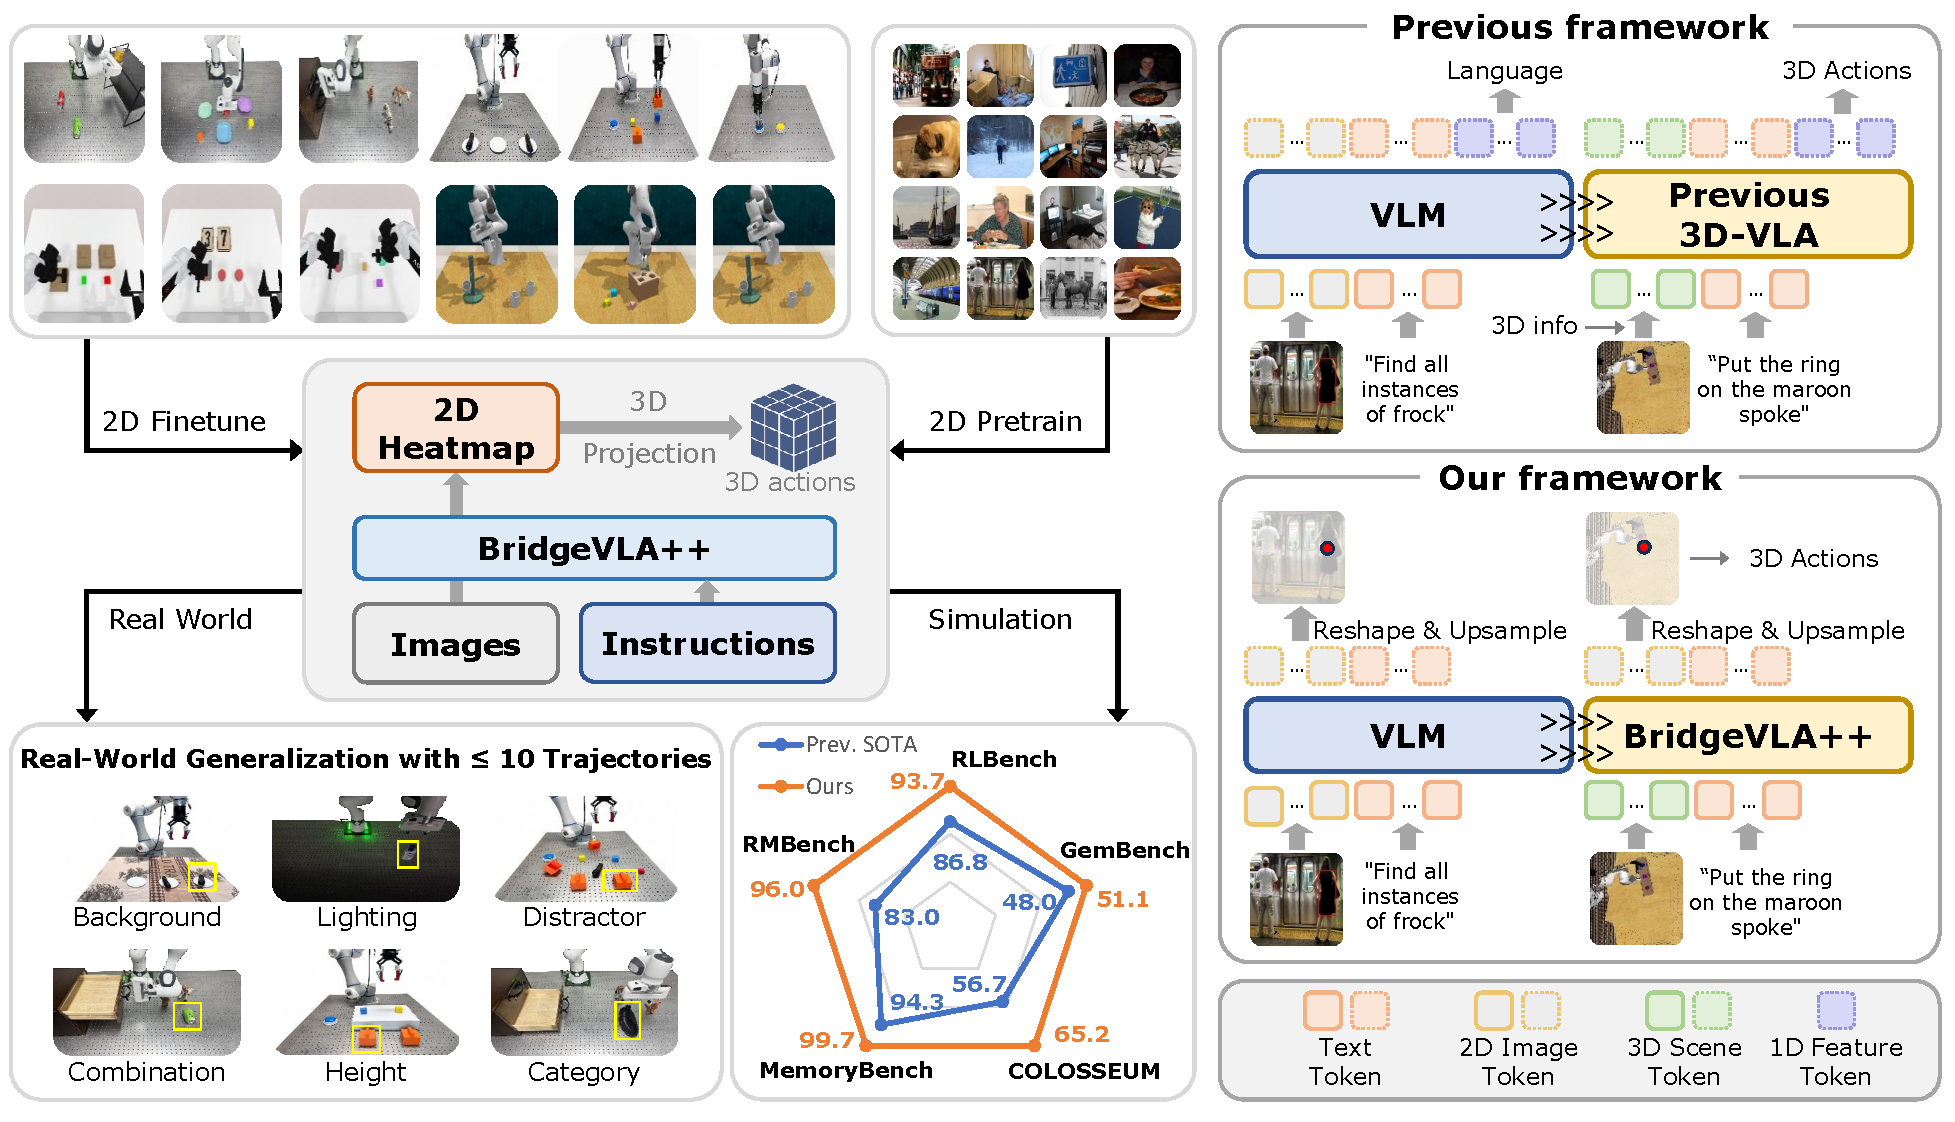
\includegraphics[width=\linewidth]{figures/teaser.pdf}
  \caption{\textbf{Overview.}
  \method\ is a 3D VLA framework that aligns its inputs and outputs in a
  unified 2D image space. It is pre-trained on object grounding using 2D heatmaps
  and fine-tuned on action prediction for 3D manipulation.
  \memmethod extends \method with a unified spatio-temporal memory architecture
  in which temporal memory preserves interaction history to determine
  \emph{what to do next}, whereas spatial memory restores previously observed
  geometry to determine \emph{where exactly to act}.
  Experiments in both simulated and real-world settings demonstrate that
  \memmethod effectively handles memory-dependent and memory-free tasks while
  preserving \method's data efficiency and generalization capabilities.}
  \label{fig:teaser}
\end{figure*}

\IEEEPARstart{L}{everaging} pre-trained vision-language models (VLMs) to
construct vision-language-action (VLA) models has become a promising
approach to learning generalizable and robust robot manipulation policies
\cite{kimopenvla,intelligence2025pi_,yu2026wall,li2023vision,brohan2023rt}.
However, most VLA models operate on 2D images and require large amounts of
robot data.
In contrast, 3D manipulation policies exploit geometric
structure and achieve higher sample efficiency
\cite{shridhar2023perceiver,3d-da,gervet2023act3d,goyal2023rvt,goyal2024rvt}.
This raises a question: can a unified 3D VLA model combine the
semantic generalization of pre-trained VLMs with the geometric efficiency
of 3D manipulation policies?

Existing attempts to build 3D VLAs do not fully resolve this challenge
\cite{zhen20243d,qu2025spatialvla}.
Many methods encode actions as token sequences and predict them
autoregressively, thereby discarding the spatial correspondence between 3D
observations and actions that underlies the efficiency of prior 3D policies.
Moreover, introducing 3D inputs into a VLM creates a
modality gap from its 2D image pre-training.
The resulting misalignment limits both the transfer of VLM
priors and the exploitation of explicit 3D structure.

Beyond data efficiency and generalization, memory presents an additional
challenge.
Most VLA and 3D manipulation policies predict each action primarily from the
current observation.
They therefore struggle when the correct action depends on previous
interactions or when task-relevant geometry observed earlier becomes
occluded during execution.
A capable 3D VLA should retain both temporal task context and persistent
spatial information while preserving its original data efficiency and
generalization ability.

To address the first two challenges, our previous work introduced
\method, a 3D VLA framework based on input--output alignment.
\method projects point-cloud observations into multi-view orthographic
images \cite{goyal2023rvt,goyal2024rvt} and processes them with a
pre-trained VLM.
Instead of predicting actions as tokens, it predicts a 2D translational
heatmap for each view and back-projects the heatmap maxima into a 3D
end-effector position.
A scalable object-grounding pre-training stage further teaches the VLM to
predict language-conditioned heatmaps before robot-policy fine-tuning.
As a result, both pre-training and downstream manipulation are performed in
the same 2D visual-localization space, enabling data-efficient and
generalizable 3D action learning.

In this article, we extend \method into \memmethod by introducing a unified
spatio-temporal memory architecture.
The temporal memory maintains selected historical observations, allowing the policy to distinguish visually similar
situations occurring at different task stages and to determine
\emph{what to do next}.
The spatial memory preserves geometric information from an earlier,
less-occluded observation and re-renders the stored scene, recovering target regions that may be hidden by the robot or manipulated objects and helping the policy
determine \emph{where exactly to act}.
Such scene-level memory representation can also be shared across two arms,
enabling a natural extension to bimanual manipulation with a common backbone
and arm-specific action heads.

We evaluate \method and \memmethod on five simulation benchmarks.
The original \method achieves state-of-the-art performance on
RLBench \cite{james2020rlbench},
COLOSSEUM \cite{pumacay2024colosseum}, and
GemBench \cite{garcia2024towards}, demonstrating strong sample efficiency
and out-of-distribution generalization.
With the proposed memory architecture, \memmethod establishes
state-of-the-art results on two memory-dependent benchmarks,
RMBench \cite{chen2026rmbench} and
MemoryBench \cite{fang2025sam2act}.
\memmethod matches or improves upon \method on the original
benchmarks, showing that memory-dependent reasoning is gained without
sacrificing its original performance.

We further validate the framework on two real-world robot embodiments,
Franka Research 3 and Dobot CR5A, covering both memory-independent and memory-dependent tasks.
On memory-independent tasks, \method outperforms a strong baseline by
32\% on average and remains robust under visual perturbations, unseen object
categories, and unseen instructions.
On memory-dependent tasks, \memmethod improves the average success rate from
20.0\% to 93.3\% over \method.
These results demonstrate that the proposed extension has cross-embodiment scalability while preserving the
data efficiency and generalization ability of the original framework.

The main contributions of this article are summarized as follows:
\begin{itemize}
  \item We present \method, a data-efficient and generalizable 3D VLA
  framework that aligns VLM pre-training and 3D manipulation learning in a
  shared  2D heatmap space.

  \item We introduce a scalable language-conditioned heatmap pre-training
  strategy that transfers object-grounding knowledge to downstream robot
  action prediction.

  \item We propose \memmethod, a unified spatio-temporal memory architecture
  that combines temporal interaction history and persistent spatial
  information to determine both \emph{what to do next} and
  \emph{where exactly to act}.

  \item We conduct extensive experiments on five simulation benchmarks and
  two real-world robot embodiments, demonstrating state-of-the-art
  performance, strong data efficiency and generalization, bimanual manipulation, effective
  memory-dependent reasoning, and
  cross-embodiment scalability.
\end{itemize}

This article is an extension to our NeurIPS 2025 conference paper
\cite{li2026bridgevla}.
The major extensions are:
\begin{itemize}
  \item a unified spatio-temporal memory architecture that equips
  \method with explicit memory-dependent reasoning;

  \item evaluation on two additional memory-dependent benchmarks,
  RMBench and MemoryBench;

  \item an extension from single-arm to bimanual manipulation;

  \item new real-world experiments on different embodiments and tasks, together with
  additional analyses showing that the memory extension preserves the data
  efficiency and generalization ability of the original framework.
\end{itemize}

The remainder of this article is organized as follows.
Sec.~\ref{sec:related_work} reviews related work.
Sec.~\ref{sec:bridgevla} introduces the original \method framework,
and Sec.~\ref{sec:memmethod} presents the proposed \memmethod
architecture.
Sec.~\ref{sec:experiments} reports simulation and real-world
experiments together with ablation studies.
Finally, Sec.~\ref{sec:conclusion} concludes the article.
Implementation and evaluation details are provided in
Appendices~\ref{app:arch_details}--\ref{app:compute_resources}, and the
full experimental results in
Appendices~\ref{app:colosseum_results}--\ref{app:real_settings_vis}.